\documentclass[border=0pt]{standalone}
\usepackage[left=25mm,right=25mm,top=25mm,bottom=25mm]{geometry}
\usepackage[utf8]{inputenc}
\usepackage[T1]{fontenc}
\usepackage{times}
\usepackage{geometry}
\usepackage{amsmath}
\usepackage{amssymb}
\usepackage{mathrsfs}
\usepackage{amsfonts}
\usepackage{amsthm}
\usepackage{lipsum}
\usepackage{amscd}
\usepackage{graphicx}
\usepackage{fancyhdr}
\usepackage{textcomp}
\usepackage{txfonts}
\usepackage[all]{xy}
\usepackage{paralist}
\usepackage[colorlinks=true]{hyperref}
\usepackage{array}
\usepackage{tikz}
\usepackage{slashed}
\usepackage{pdfpages}
\usepackage{cite}
\usepackage{url}

\usepackage{listings}
\usepackage{multirow}
\usepackage{color}

\begin{document}



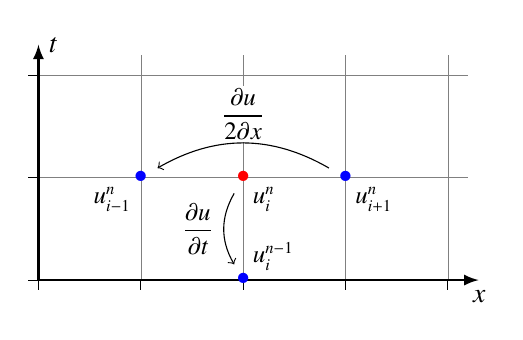
\begin{tikzpicture}[scale=1.3]
 %  \draw[thick,step=1cm,help lines] (0,0) grid (3,3);
 %  %\draw[ultra thin,step=.5cm,help lines] (0,0) grid (5,5);
 %  % Draw axes
 %  \draw[thick,-latex] (0,0) -- (3.3,0) node[anchor=north](){x};
 %  \draw[thick,-latex] (0,0) -- (0,3.3) node[anchor= west](){t};
 %  % the co-ordinates -- major
 %  \foreach \x in {0,1,...,3}  {   % for x-axis
 %  \draw [] (\x,0) -- (\x,0.1);
 %  }
 %  \foreach \y in {0,1,...,3} {   %% for y-axis
 %  \draw [] (0,\y) -- (-0.1,\y);
 %  }
 %  % the numbers
 %  \foreach \x in {0,1,...,3} { \node [anchor=center] at (\x, -0.2) {\tiny \x}; }
 %  % \foreach \y in {0,1,...,3} { \node [anchor=center] at (-0.2,-\y) {\tiny \y}; }
 %
 % \node [anchor=center] at (-.3,1) {\tiny $u^n$};
 % \node [anchor=center] at (-.3,2) {\tiny $u^{n+1}$};
 % % \foreach \x in {0,1,...,3} {  \draw (\x,2)[fill=black] circle [radius=0.03]; }
 % \foreach \x in {0,1,...,3} {  \draw (\x,1)[fill=black] circle [radius=0.08]; }
 %
 % \draw (0,2)[red, fill=red] circle [radius=0.08];
 % \draw (1,2)[blue, fill=blue] circle [radius=0.08];
 % \draw (2,2)[green, fill=green] circle [radius=0.08];
 % \draw (3,2)[orange, fill=orange] circle [radius=0.08];
 %
 % \draw (0,1)[thick,red] circle [radius=0.12];
 % % \draw (0,2)[red] circle [radius=0.05];
 % \draw (1,2)[thick,red] circle [radius=0.12];
 % %
 % \draw (1,1)[thick,blue] circle [radius=0.12];
 % \draw (0,2)[thick,blue] circle [radius=0.12];
 % \draw (2,2)[thick,blue] circle [radius=0.12];
 % % \draw (1,2)[blue] circle [radius=0.07];
 % %
 % \draw (2,1)[thick,green] circle [radius=0.12];
 % \draw (1,2)[thick,green] circle [radius=0.145];
 % \draw (3,2)[thick,green] circle [radius=0.12];
 % % \draw (2,2)[orange] circle [radius=0.07];
 % %
 % \draw (3,1)[thick, orange] circle [radius=0.12];
 % % \draw (3,2)[green] circle [radius=0.05];
 % \draw (2,2)[thick,orange] circle [radius=0.145];


 \draw[thick,step=1cm,help lines] (0,0) grid (4.2,2.2);
 %\draw[ultra thin,step=.5cm,help lines] (0,0) grid (5,5);
 % Draw axes
 \draw[thick,-latex] (0,0) -- (4.3,0) node[anchor=north](){$x$};
 \draw[thick,-latex] (0,0) -- (0,2.3) node[anchor= west](){$t$};
 % the co-ordinates -- major
 \foreach \x in {0,1,...,4}  {   % for x-axis
 \draw [] (\x,0) -- (\x,-0.1);
 }
 \foreach \y in {0,1,...,2} {   %% for y-axis
 \draw [] (0,\y) -- (-0.1,\y);
 }
 % the numbers
 % \foreach \x in {0,1,...,3} { \node [anchor=center] at (\x,0.2) {\tiny \x}; }
 % \foreach \y in {0,1,...,3} { \node [anchor=center] at (-0.2,-\y) {\tiny \y}; }

 \draw (2,1) node[red, anchor=center](1){\textbullet};
 \draw (2,1) node[anchor=north west]{\small$u_{i}^{n}$};
 \draw (3,1) node[blue, anchor=center](3){\textbullet};
 \draw (3,1) node[anchor=north west]{\small$u_{i+1}^{n}$};
 \draw (1,1) node[blue, anchor=center](4){\textbullet};
 \draw (1,1) node[anchor=north east]{\small$u_{i-1}^{n}$};
 \draw (2,0) node[blue, anchor=center](5){\textbullet};
 \draw (2,0) node[anchor=south west]{\small$u_{i}^{n-1}$};
 \draw [->] (3) to [out=150,in=30]node[anchor=south, fill=white,inner sep=.9pt]{{\small $\displaystyle \frac{\partial u}{2\partial x}$}} (4);
 \draw [->] (1) to [out=240,in=120]node[anchor=east]{ \small $\displaystyle \frac{\partial u}{\partial t}$} (5) ;


\end{tikzpicture}




\end{document}
